\section{Frontend}
Das Frontend definiert eine Webpage als Schnittstelle zwischen Anwendern und Dienst, sowie Verwaltungsmöglichkeiten für Administratoren bietet. Zur Navigation bzw Suche von Interfaces und Components werden eine Gesamtliste sowie eine Suchfunktion zur Verfügung gestellt. Es betreibt außerdem eine Datenbank in der alle nötigen Daten gespeichert werden.

\subsection{Use-Cases}

\begin{figure}[!htp]
\begin{center}
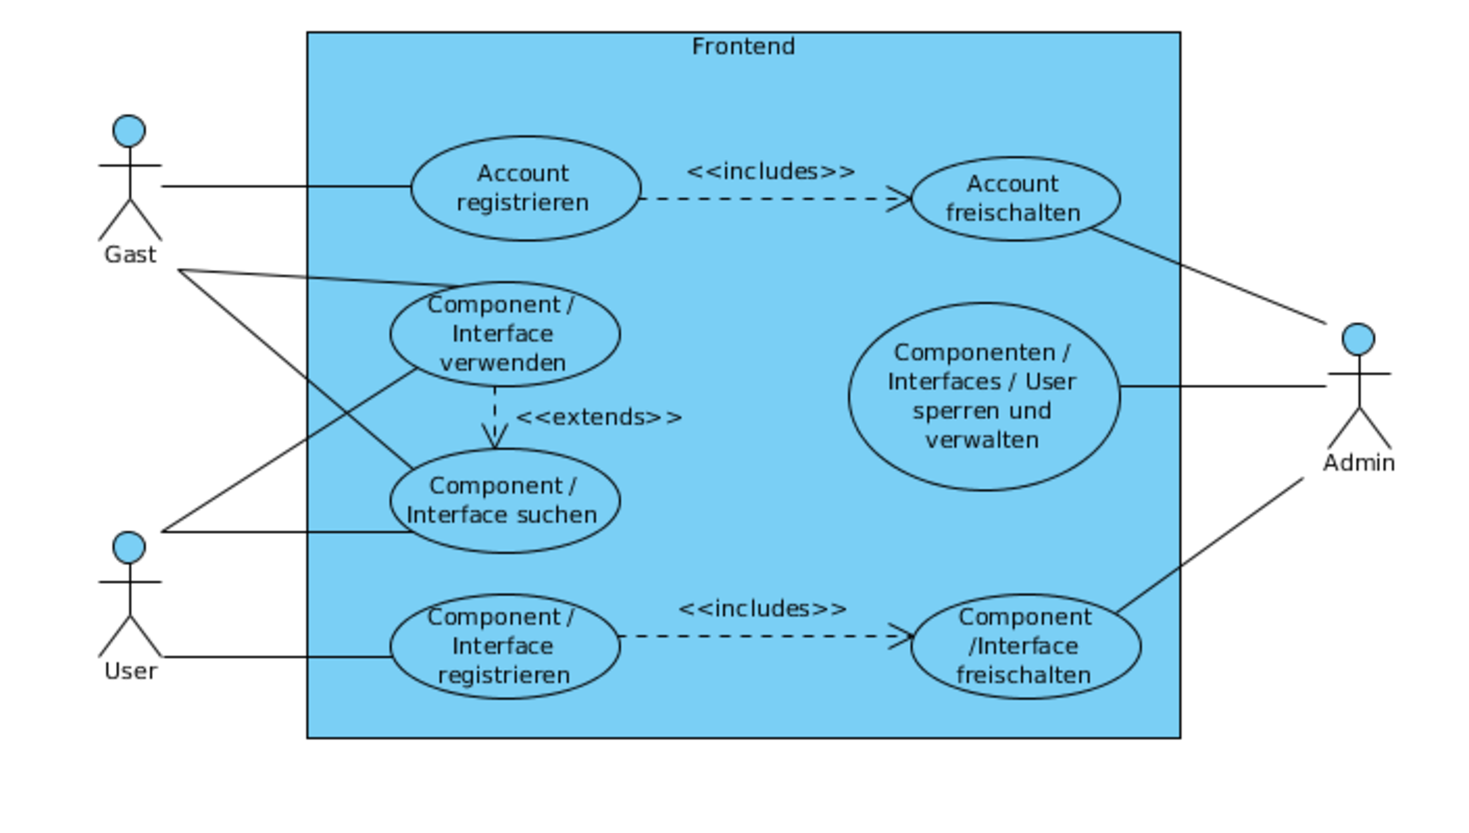
\includegraphics[width=\textwidth]{bilder/use_case_frontend.pdf}
\caption{Use-Case-Diagramm des Frontend}
\label{fig:uc_front}
\end{center}
\end{figure}

Erklärung des Use-Case-Diagramm \ref{fig:uc_front}
1) Ein Gast kann einen Account registrieren. Dieser Account muss daraufhin von einem Admin freigeschaltet werden. Außerdem kann ein Gast eine Component suchen.\\
2) Ein User (mit registriertem Account) kann zusätzlich zum Suchen eine Component auch in sein Programm einbinden und verwenden. Zusätzlich ist es ihm möglich eigenen Components/Interfaces zur Verfügung zu stellen. Bevor diese Components/Interfaces benutzt werden können, müssen sie von einem Admin freigeschaltet werden.\\
3)Zusätzlich zu den bereits angegebenen Funktionen des Freischaltens hat ein Admin die Möglichkeit User/Components/Interfaces zu verwalten bzw. zu sperren.\\

\subsection{Datenbankmodell}

\begin{figure}[H]
  \begin{center}
	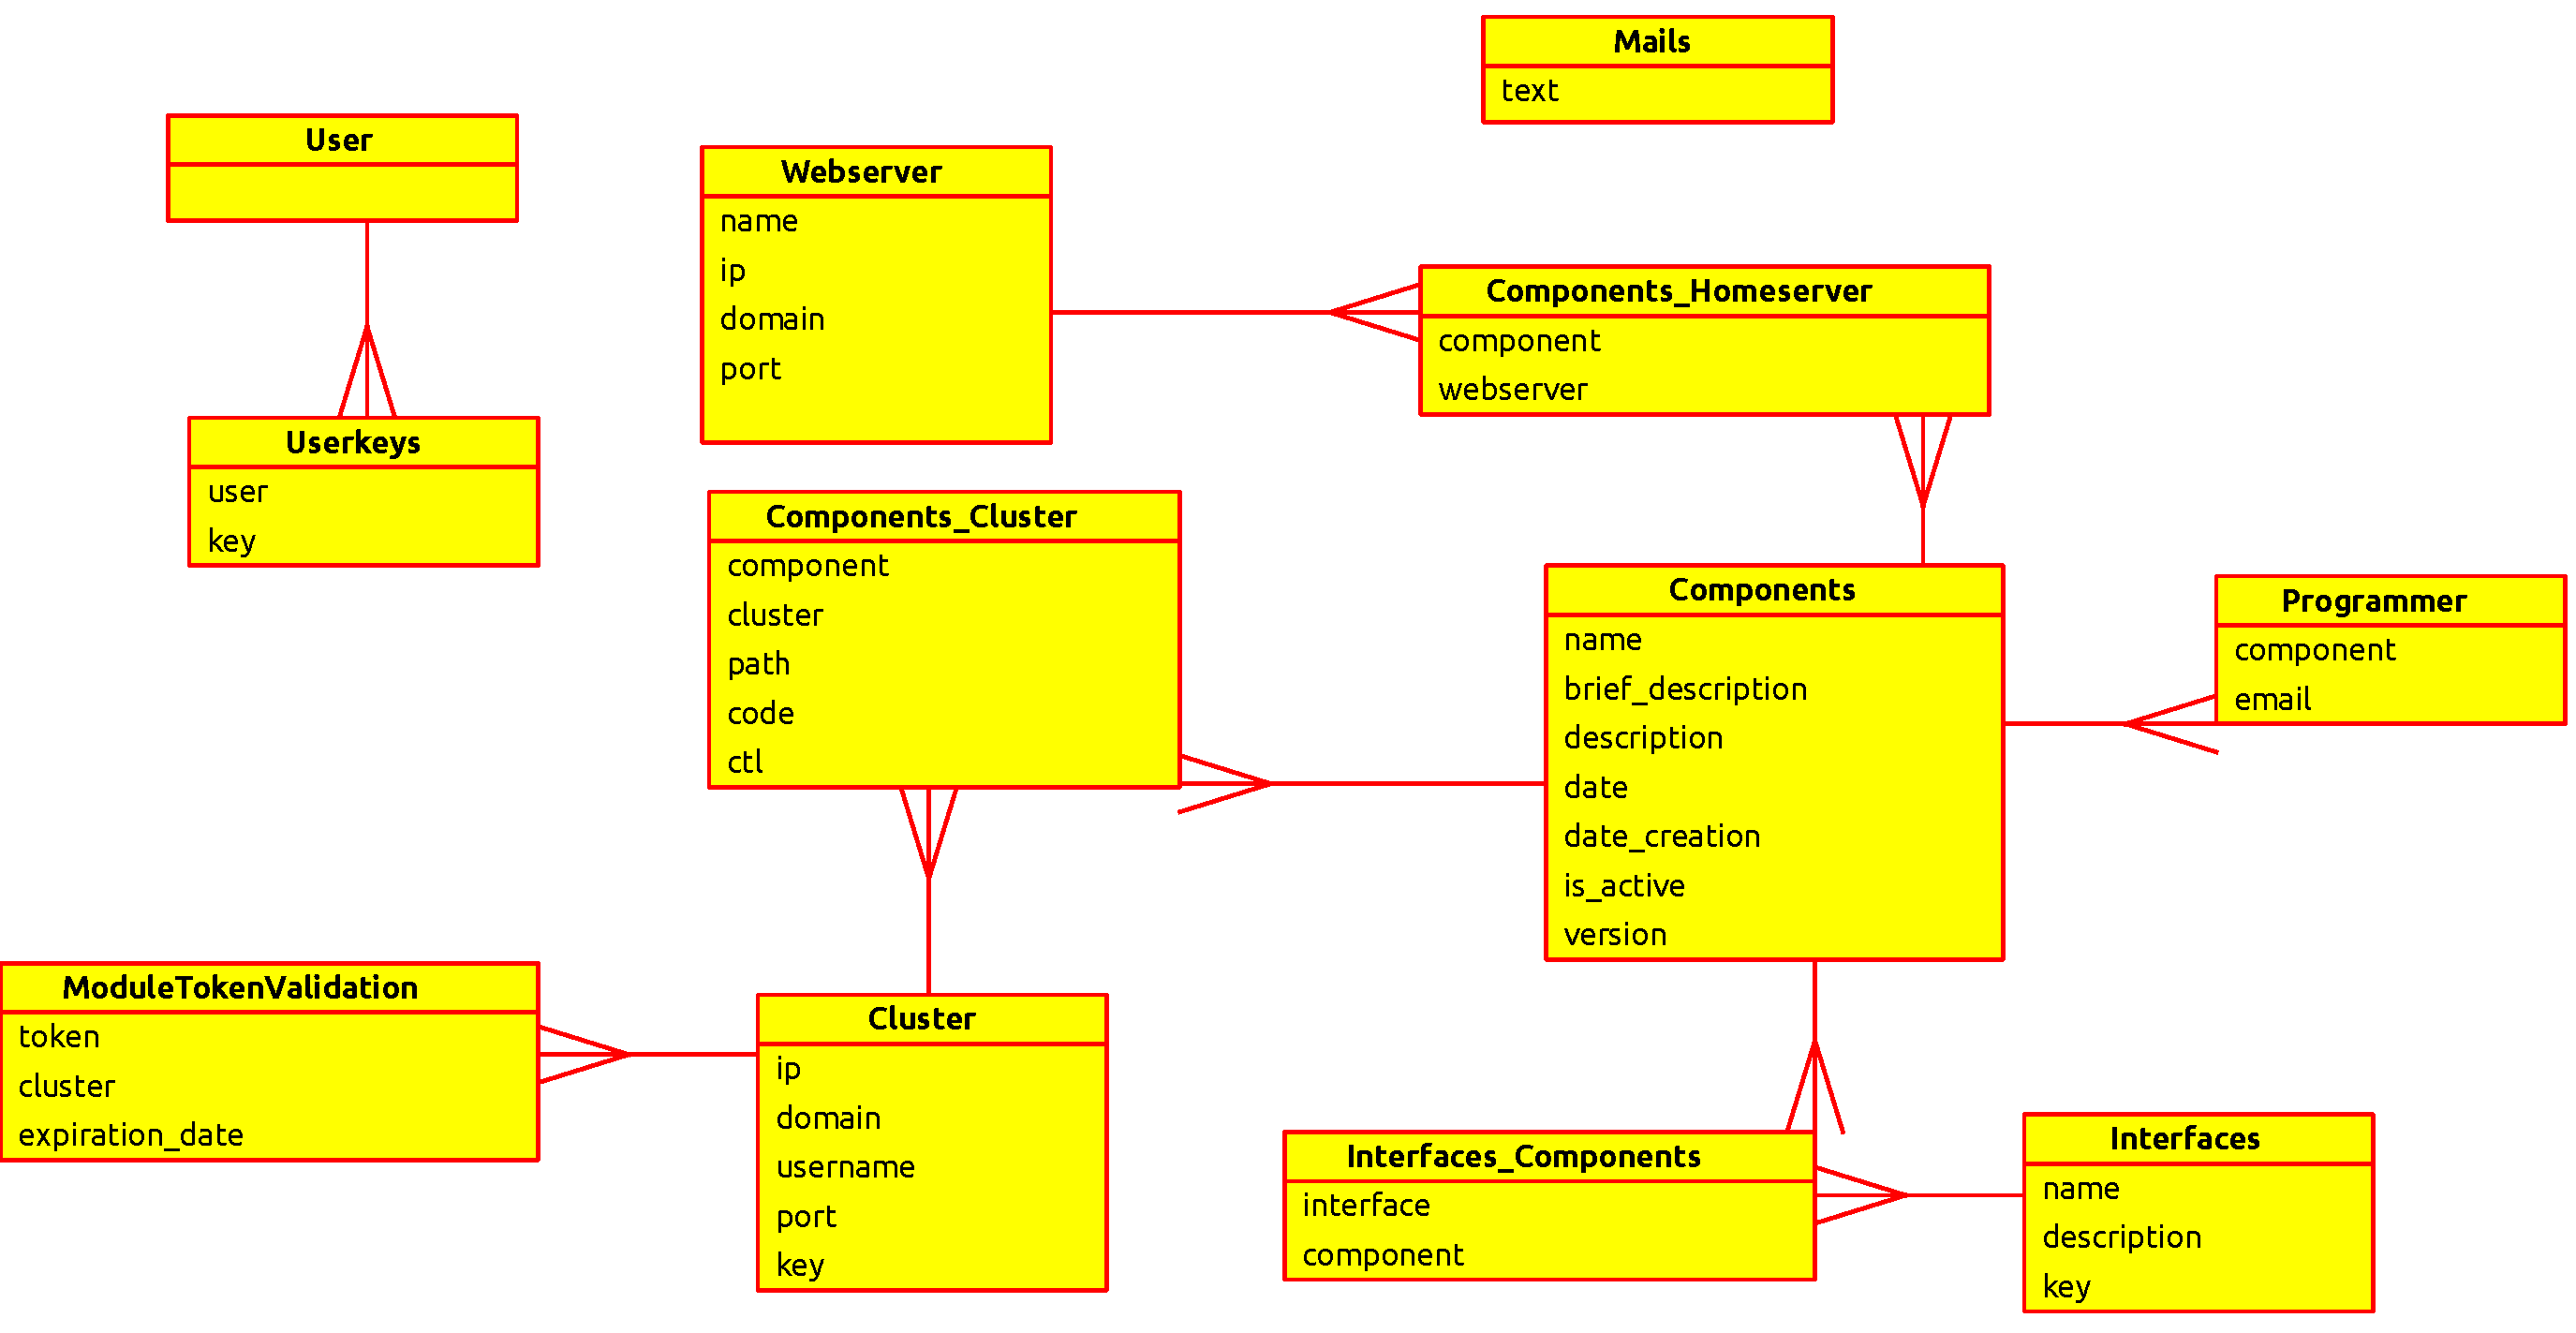
\includegraphics[width=\linewidth]{bilder/ctl-db.pdf}
	\caption{Modell der Frontend-Datenbank}
	\label{fb_db}
  \end{center}
\end{figure}

In \ref{fb_db} ist die Datenbank des Frontends modellartig dargestellt. Dabei
gibt es zwei kleinere Abschnitte; zum Einen ist es die Userverwaltung und zum
Anderen die Verwaltung der Componenten. 

Bei der Userverwaltung wurden die Standarts von Django
\footnote{\url{https://docs.djangoproject.com}} genutzt. Dazu wurden eine
weitere Tabelle erstellt, welchem jeden User bestimmte Keys zuordnet
(\textbf{Userkeys}) und damit beide Felder zusammen unique sind, und eine, in 
der Mails abgespeichert werden können (\textbf{Mails}).

Zur Componentenverwaltung gehören \textbf{Webserver}, \textbf{Cluster},
\textbf{ModuleTokenValidation}, \textbf{Interfaces}, \textbf{Programmer}, 
\textbf{Components} sowie einige Verbindungstabellen.
Falls in der folgenden Beschreibung keine PK angegeben ist, existiert ein PK
namens \textit{id}. 

\begin{description}
  \item[\textbf{Cluster}]
	Sämtliche Felder dieser Klasse dürfen den Wert \glqq null\grqq\ annehmen.
	Allerdings sind \textit{ip} und \textit{domain} zusammen unique.
  \item[\textbf{Components}]
	Die Spalte \textit{name} ist unique. In \textit{date} wird das Datum der
	letzten Änderung abgespeichert und in \textit{date\_creation} das
	Erstellungsdatum. Die \textit{brief\_description} darf im Übrigen nur 255
	Zeichen lang sein.
  \item[\textbf{Components\_Cluster}]
	Dies ist die Verbindungstabelle zwischen \textbf{Cluster} und
	\textbf{Compo\-nents}. Dabei wird jeweils der Speicherpfad (\textit{path}),
	den Quellcode (\textit{code}) und den ctl-\,Befehl (\textit{ctl}). Dabei
	wird der ctl-\,Befehl beim Speichern automatisch generiert.
  \item[\textbf{Interfaces}]
	Diese Tabelle hat ein PK - \textit{key}. Außerdem ist \textit{name} unique.
  \item[\textbf{Programmer}]
	Die beiden Spalten \textit{component} - FK zu \textbf{Components} - und
	\textit{email} sind zusammen unique. 
  \item[\textbf{Webserver}]
	Hier können \textit{ip}, \textit{domain} und \textit{port} alle den Wert
	\glqq null\grqq\ annehmen. Die ersten beiden von denen sind allerdings
	zusammen unique.
\end{description}
